\documentclass{beamer}
% Thesis defense deck prepared for the oral presentation.
\usepackage[utf8]{inputenc}
\usepackage[T1]{fontenc}
\usepackage{amsfonts,amsmath}
\usepackage{array,booktabs,colortbl}
\usepackage{graphicx}
\usepackage{tikz}
\usepackage{url}
\usetikzlibrary{arrows.meta,positioning,calc,fit}
\usetheme{sintef}
\usefonttheme[onlymath]{serif}

% This defense deck uses a continuous narrative; suppress the theme's
% automatic table-of-contents frame at each section boundary.
\AtBeginSection[]{}

\titlebackground*{assets/background}

\setbeamerfont{frametitle}{size=\Large,series=\bfseries}
\setbeameroption{hide notes}

\newcommand{\highlight}[1]{\textcolor{maincolor}{\textbf{#1}}}
\newcommand{\slideNote}[2]{%
  \note{\textbf{Presentation cue:} #1\par\medskip
  \textbf{[Sources]}\par #2}%
}

\tikzset{
  panel/.style={
    rounded corners=3pt,
    draw=maincolor!25,
    line width=0.6pt,
    fill=white,
    inner sep=7pt,
    align=center
  },
  softpanel/.style={
    rounded corners=3pt,
    draw=maincolor!25,
    line width=0.6pt,
    fill=maincolor!6,
    inner sep=7pt,
    align=center
  },
  greenpanel/.style={
    rounded corners=3pt,
    draw=sintefgreen!75!black,
    line width=0.7pt,
    fill=sinteflightgreen,
    inner sep=7pt,
    align=center
  },
  amberpanel/.style={
    rounded corners=3pt,
    draw=sintefyellow!80!black,
    line width=0.7pt,
    fill=sintefyellow!16,
    inner sep=7pt,
    align=center
  },
  redpanel/.style={
    rounded corners=3pt,
    draw=sintefred!80!black,
    line width=0.7pt,
    fill=sintefred!10,
    inner sep=7pt,
    align=center
  },
  darkpanel/.style={
    rounded corners=4pt,
    draw=maincolor,
    fill=maincolor,
    inner sep=8pt,
    align=center
  },
  flowarrow/.style={
    ->,
    >=Stealth,
    line width=0.9pt,
    draw=maincolor!80
  }
}

\title{Evaluating the Robustness of AI-Based Forensic Tools under Adversarial and Anti-Forensic Attacks}
\course{Master's Degree in Computer Engineering, Cybersecurity and Artificial Intelligence}
\author{Lello Molinario}
\IDnumber{70/90/00369}
\advisor{Prof. Davide Maiorca}
\coadvisor{Silvia Lucia Sanna, Ph.D.}
\date{Academic Year 2025/2026}
\footlinepayoff{Lello Molinario \enspace$\vert$\enspace MSc Thesis Defense}

\begin{document}

% ---------------------------------------------------------------------
% 01 — Title
% ---------------------------------------------------------------------
\begingroup
\setbeamertemplate{background}{\TikzSplitSlide{assets/background}}
\begin{frame}[plain]
  \titlepage
  \slideNote
    {Introduce the thesis as an operational robustness study, not as a new firearm classifier.}
    {\url{../LatexThesis/title.tex}\par
     \url{../LatexThesis/sections/00_abstract.tex}}
\end{frame}
\endgroup

% ---------------------------------------------------------------------
\section{Question and protocol}
% ---------------------------------------------------------------------

% 02 — Operational question
\begin{frame}{The operational risk is silent exclusion}
\centering
\begin{tikzpicture}[x=1cm,y=1cm]
  % Connectors first so that they remain behind the panels.
  \draw[flowarrow,line width=1.1pt] (-2.48,1.55) -- (-1.62,1.55);
  \draw[flowarrow,line width=1.1pt] (1.62,1.55) -- (2.48,1.55);

  \node[panel,minimum width=3.25cm,minimum height=1.55cm] at (-4.10,1.55) {
    {\fontsize{24}{26}\selectfont\bfseries\color{maincolor}LARGE}\\[-0.02cm]
    {\small image collections}
  };
  \node[softpanel,minimum width=3.25cm,minimum height=1.55cm] at (0,1.55) {
    {\fontsize{24}{26}\selectfont\bfseries\color{maincolor}AI}\\[-0.02cm]
    {\small assisted triage}
  };
  \node[redpanel,minimum width=3.25cm,minimum height=1.55cm] at (4.10,1.55) {
    {\fontsize{24}{26}\selectfont\bfseries\color{sintefred!90!black}MISS}\\[-0.02cm]
    {\small relevant evidence}
  };

  \node[darkpanel,minimum width=12.20cm,minimum height=1.28cm] at (0,-0.12) {
    {\large\bfseries\color{white}How does forensic image triage behave under}\\[-0.01cm]
    {\large\bfseries\color{white}adversarial, anti-forensic and OOD inputs?}
  };

  \node[font=\small,align=center,text=black!70,text width=11.5cm] at (0,-1.40) {
    Clean accuracy can look reassuring while a relevant item is quietly moved out of the analyst's priority queue.
  };

  \node[greenpanel,minimum width=11.30cm,minimum height=0.68cm,
        font=\scriptsize\bfseries,text width=10.65cm] at (0,-2.30) {
    Contribution: auditable robustness assessment---not a new firearm classifier.
  };
\end{tikzpicture}
\slideNote
  {Start from the operational risk: the relevant error is a missed item that disappears from the analyst's priority queue.}
  {\url{../LatexThesis/sections/01_introduction.tex}\par
   \url{../LatexThesis/sections/04_methodology.tex}}
\end{frame}

% 03 — FAIRLab
\begin{frame}{FAIRLab makes robustness auditable}
\centering
\begin{tikzpicture}[x=1cm,y=1cm]
  % Six stages adapted from the publication workflow, with final thesis counts.
  \draw[flowarrow] (-2.30,1.48) -- (-2.00,1.48);
  \draw[flowarrow] (2.00,1.48) -- (2.30,1.48);
  \draw[flowarrow] (4.18,0.55) -- (4.18,0.24);
  \draw[flowarrow] (2.30,-0.72) -- (2.00,-0.72);
  \draw[flowarrow] (-2.00,-0.72) -- (-2.30,-0.72);

  \node[panel,minimum width=3.40cm,minimum height=1.42cm] at (-4.18,1.48) {
    {\scriptsize\bfseries\color{maincolor}01 · SOURCE}\\[0.06cm]
    {\small\bfseries heterogeneous pool}
  };
  \node[greenpanel,minimum width=3.40cm,minimum height=1.42cm] at (0,1.48) {
    {\scriptsize\bfseries\color{maincolor}02 · VALIDATE}\\[0.06cm]
    {\small\bfseries review + dedup}
  };
  \node[softpanel,minimum width=3.40cm,minimum height=1.42cm] at (4.18,1.48) {
    {\scriptsize\bfseries\color{maincolor}03 · FREEZE}\\[0.06cm]
    {\small\bfseries 1,500 sources}
  };
  \node[amberpanel,minimum width=3.40cm,minimum height=1.42cm] at (4.18,-0.72) {
    {\scriptsize\bfseries\color{maincolor}04 · PERTURB}\\[0.06cm]
    {\small\bfseries 10,000 variants}
  };
  \node[panel,minimum width=3.40cm,minimum height=1.42cm] at (0,-0.72) {
    {\scriptsize\bfseries\color{maincolor}05 · EVALUATE}\\[0.06cm]
    {\small\bfseries 3 proxies + 6 configs}
  };
  \node[greenpanel,minimum width=3.40cm,minimum height=1.42cm] at (-4.18,-0.72) {
    {\scriptsize\bfseries\color{maincolor}06 · INTERPRET}\\[0.06cm]
    {\small\bfseries normalize + interpret}
  };

  \node[darkpanel,minimum width=12.15cm,minimum height=0.84cm,
        font=\scriptsize,text width=11.55cm] at (0,-2.15) {
    {\bfseries\color{sintefgreen}TRACEABILITY THROUGHOUT}\\[-0.01cm]
    {\color{white}deterministic IDs · manifests · checksums · frozen configurations · source-to-output links}
  };
\end{tikzpicture}
\slideNote
  {Explain FAIRLab as the protocol that connects data provenance, controlled perturbations and normalized decisions.}
  {\url{../LatexThesis/sections/04_methodology.tex}\par
   \url{../LatexThesis/sections/05_implementation.tex}}
\end{frame}

% 04 — Dataset
\begin{frame}{One population becomes 11,500 traceable files}
\centering
\begin{tikzpicture}[x=1cm,y=1cm]
  \node[font=\fontsize{28}{30}\selectfont\bfseries,text=maincolor] at (0,2.43)
    {1,500 SOURCE IMAGES};

  \node[redpanel,minimum width=3.55cm,minimum height=1.30cm] at (-4.20,1.15) {
    {\fontsize{23}{25}\selectfont\bfseries\color{sintefred!90!black}500}\\[-0.01cm]
    {\small\bfseries weapon}
  };
  \node[greenpanel,minimum width=3.55cm,minimum height=1.30cm] at (0,1.15) {
    {\fontsize{23}{25}\selectfont\bfseries\color{sintefgreen!60!black}500}\\[-0.01cm]
    {\small\bfseries non-weapon}
  };
  \node[amberpanel,minimum width=3.55cm,minimum height=1.30cm] at (4.20,1.15) {
    {\fontsize{23}{25}\selectfont\bfseries\color{sintefyellow!70!black}500}\\[-0.01cm]
    {\small\bfseries separate OOD branch}
  };

  \node[softpanel,minimum width=7.15cm,minimum height=1.48cm] at (-2.72,-0.62) {
    {\fontsize{23}{25}\selectfont\bfseries\color{maincolor}1,000 $\times$ 10 = 10,000}\\[-0.01cm]
    {\small linked adversarial and anti-forensic variants}
  };
  \node[darkpanel,minimum width=4.55cm,minimum height=1.48cm] at (4.12,-0.62) {
    {\fontsize{25}{27}\selectfont\bfseries\color{white}11,500}\\[-0.01cm]
    {\small\bfseries\color{sintefgreen}tool-facing files}
  };

  \node[font=\scriptsize\bfseries,text=black!62,align=center,text width=11.7cm] at (0,-1.87) {
    The 10,000 manipulated files are linked source--condition variants---not 10,000 independent cases.
  };
  \node[font=\scriptsize,text=black!58,align=center,text width=11.7cm] at (0,-2.35) {
    OOD is evaluated separately and is not treated as a third supervised class.
  };
\end{tikzpicture}
\slideNote
  {Clarify the denominator: the frozen corpus contains 1,500 source images; manipulated files are controlled variants.}
  {\url{../LatexThesis/sections/04_methodology.tex}\par
   \url{../LatexThesis/sections/05_implementation.tex}}
\end{frame}

% 05 — Evidence levels
\begin{frame}{Two evidence levels, one frozen corpus}
\centering
\begin{tikzpicture}[x=1cm,y=1cm]
  \node[softpanel,minimum width=6.10cm,minimum height=2.18cm,align=left,text width=5.35cm] at (-3.45,1.35) {
    {\small\bfseries\color{maincolor}TRANSPARENT PROXIES}\\[0.13cm]
    {\small\bfseries EfficientNet-B0 (attack source)}\\[0.02cm]
    {\small\bfseries ResNet18 · CLIP proxy}\\[0.11cm]
    {\scriptsize\color{black!60}Predictions, gradients and checkpoints are visible}
  };

  \node[panel,minimum width=6.10cm,minimum height=2.18cm,align=left,text width=5.35cm] at (3.45,1.35) {
    {\small\bfseries\color{maincolor}BLACK-BOX SOFTWARE}\\[0.04cm]
    {\scriptsize\bfseries\color{maincolor}4 systems · 6 configurations}\\[0.10cm]
    {\small\bfseries Magnet.AI · Excire D20/D50/D80}\\[0.02cm]
    {\small\bfseries Cellebrite · Griffeye/T3K}\\[0.10cm]
    {\scriptsize\color{black!60}Only exported decisions are observable}
  };

  \node[redpanel,minimum width=3.95cm,minimum height=1.28cm,text width=3.35cm] at (-4.35,-1.40) {
    {\scriptsize\bfseries\color{sintefred!90!black}DIRECT TARGET}\\[0.07cm]
    {\scriptsize Model-dependent attacks on EfficientNet-B0}
  };
  \node[amberpanel,minimum width=3.95cm,minimum height=1.28cm,text width=3.35cm] at (0,-1.40) {
    {\scriptsize\bfseries\color{sintefyellow!70!black}EMPIRICAL TRANSFER}\\[0.07cm]
    {\scriptsize Generated artifacts applied to non-target systems}
  };
  \node[greenpanel,minimum width=3.95cm,minimum height=1.28cm,text width=3.35cm] at (4.35,-1.40) {
    {\scriptsize\bfseries\color{sintefgreen!60!black}MODEL-AGNOSTIC}\\[0.07cm]
    {\scriptsize Color Shift + five anti-forensic transforms}
  };
\end{tikzpicture}
\slideNote
  {Keep the claim boundaries explicit: only EfficientNet-B0 receives direct model-dependent attacks; the other systems measure transfer.}
  {\url{../LatexThesis/sections/04_methodology.tex}\par
   \url{../LatexThesis/sections/06_results.tex}}
\end{frame}

% 06 — Mappings
\begin{frame}{Comparable metrics require explicit output mappings}
\centering
\begin{tikzpicture}[x=1cm,y=1cm]
  % Connectors first.
  \draw[flowarrow] (-3.60,1.54) -- (-1.85,1.54);
  \draw[flowarrow] (1.85,1.54) -- (3.60,1.54);

  \node[panel,minimum width=3.35cm,minimum height=1.45cm,text width=2.78cm] at (-5.15,1.54) {
    {\small\bfseries\color{maincolor}Observable outputs}\\[0.10cm]
    {\scriptsize tags · bookmarks\\labels · retrieval}
  };
  \node[softpanel,minimum width=3.45cm,minimum height=1.45cm,text width=2.88cm] at (0,1.54) {
    {\small\bfseries\color{maincolor}Output mapping}\\[0.10cm]
    {\scriptsize frozen per version\\and configuration}
  };
  \node[panel,minimum width=3.35cm,minimum height=1.45cm,text width=2.78cm] at (5.15,1.54) {
    {\small\bfseries\color{maincolor}Operational states}\\[0.10cm]
    {\scriptsize weapon\\non-weapon · unknown}
  };

  \draw[maincolor!18,line width=0.8pt] (0,-1.52) -- (0,0.40);

  \node[font=\small\bfseries,text=sintefred!90!black] at (-3.25,0.25) {MISSED-TARGET RISK};
  \node[font=\fontsize{34}{36}\selectfont\bfseries,text=sintefred!90!black] at (-3.25,-0.42) {FNR};
  \node[font=\small\bfseries] at (-3.25,-1.02) {weapon $\rightarrow$ non-weapon};

  \node[font=\small\bfseries,text=sintefyellow!75!black] at (3.25,0.25) {REVIEW-WORKLOAD RISK};
  \node[font=\fontsize{34}{36}\selectfont\bfseries,text=sintefyellow!75!black] at (3.25,-0.42) {FPR};
  \node[font=\small\bfseries] at (3.25,-1.02) {non-weapon $\rightarrow$ weapon};

  \node[greenpanel,minimum width=10.7cm,minimum height=0.68cm,font=\scriptsize\bfseries,text width=10.0cm] at (0,-2.10) {
    OOD weapon-assignment rate is reported separately; no unknown state occurred in 69,000 normalized decisions.
  };
\end{tikzpicture}
\slideNote
  {Define FNR as the missed-target risk and FPR as review workload. Keep OOD behavior separate from supervised false positives.}
  {\url{../LatexThesis/sections/04_methodology.tex}\par
   \url{../LatexThesis/sections/06_results.tex}}
\end{frame}

% ---------------------------------------------------------------------
\section{Results}
% ---------------------------------------------------------------------

% 07 — Proxy results
\begin{frame}{Direct-target collapse did not transfer uniformly}
\centering
\begin{tikzpicture}[x=1cm,y=1cm]
  \node[font=\scriptsize,text=black!62] at (0,2.65)
    {Worst observed adversarial condition per proxy; attacks were optimized only for EfficientNet-B0};

  \node[softpanel,minimum width=4.00cm,minimum height=4.22cm] at (-4.35,0.25) {};
  \node[softpanel,minimum width=4.00cm,minimum height=4.22cm] at (0,0.25) {};
  \node[softpanel,minimum width=4.00cm,minimum height=4.22cm] at (4.35,0.25) {};

  \node[font=\small\bfseries,text=maincolor] at (-4.35,2.03) {EfficientNet-B0};
  \node[font=\small\bfseries,text=maincolor] at (0,2.03) {ResNet18};
  \node[font=\small\bfseries,text=maincolor] at (4.35,2.03) {CLIP proxy};

  \node[font=\scriptsize\bfseries,text=black!58] at (-4.35,1.46) {CLEAN};
  \node[font=\fontsize{27}{29}\selectfont\bfseries,text=maincolor] at (-4.35,1.00) {97.8\%};
  \node[font=\scriptsize\bfseries,text=black!58] at (0,1.46) {CLEAN};
  \node[font=\fontsize{27}{29}\selectfont\bfseries,text=maincolor] at (0,1.00) {96.4\%};
  \node[font=\scriptsize\bfseries,text=black!58] at (4.35,1.46) {CLEAN};
  \node[font=\fontsize{27}{29}\selectfont\bfseries,text=maincolor] at (4.35,1.00) {92.7\%};

  \draw[-{Stealth[length=3mm]},line width=1.5pt,sintefred!85] (-4.35,0.53) -- (-4.35,-0.30);
  \draw[-{Stealth[length=3mm]},line width=1.5pt,sintefyellow!80!black] (0,0.53) -- (0,-0.30);
  \draw[-{Stealth[length=3mm]},line width=1.5pt,sintefyellow!80!black] (4.35,0.53) -- (4.35,-0.30);
  \node[font=\scriptsize\bfseries,text=sintefred!90!black] at (-3.55,0.10) {$-96.3$ pp};
  \node[font=\scriptsize\bfseries,text=sintefyellow!70!black] at (0.80,0.10) {$-4.6$ pp};
  \node[font=\scriptsize\bfseries,text=sintefyellow!70!black] at (5.15,0.10) {$-1.3$ pp};

  \node[font=\fontsize{27}{29}\selectfont\bfseries,text=sintefred!90!black] at (-4.35,-0.70) {1.5\%};
  \node[font=\fontsize{27}{29}\selectfont\bfseries,text=sintefyellow!70!black] at (0,-0.70) {91.8\%};
  \node[font=\fontsize{27}{29}\selectfont\bfseries,text=sintefyellow!70!black] at (4.35,-0.70) {91.4\%};

  \node[redpanel,minimum width=3.25cm,minimum height=0.65cm,font=\scriptsize\bfseries] at (-4.35,-1.45)
    {Sigma Zero · direct};
  \node[amberpanel,minimum width=3.25cm,minimum height=0.65cm,font=\scriptsize\bfseries] at (0,-1.45)
    {FGSM · transfer};
  \node[amberpanel,minimum width=3.25cm,minimum height=0.65cm,font=\scriptsize\bfseries] at (4.35,-1.45)
    {FGSM · transfer};

  \node[font=\scriptsize\bfseries,text=maincolor,align=center] at (0,-2.25)
    {Largest anti-forensic proxy drop: 3.0 pp (ResNet18, histogram modification).};
\end{tikzpicture}
\slideNote
  {Lead with the direct-target collapse from 97.8 percent to 1.5 percent, then separate that result from the much smaller empirical-transfer effects.}
  {\url{../../results/metrics/proxy_model_clean_metrics.csv}\par
   \url{../../results/metrics/proxy_model_adversarial_metrics.csv}\par
   \url{../../results/metrics/proxy_model_anti_forensic_metrics.csv}}
\end{frame}

% 08 — Black-box transfer
\begin{frame}{Black-box transfer was configuration-dependent}
\centering
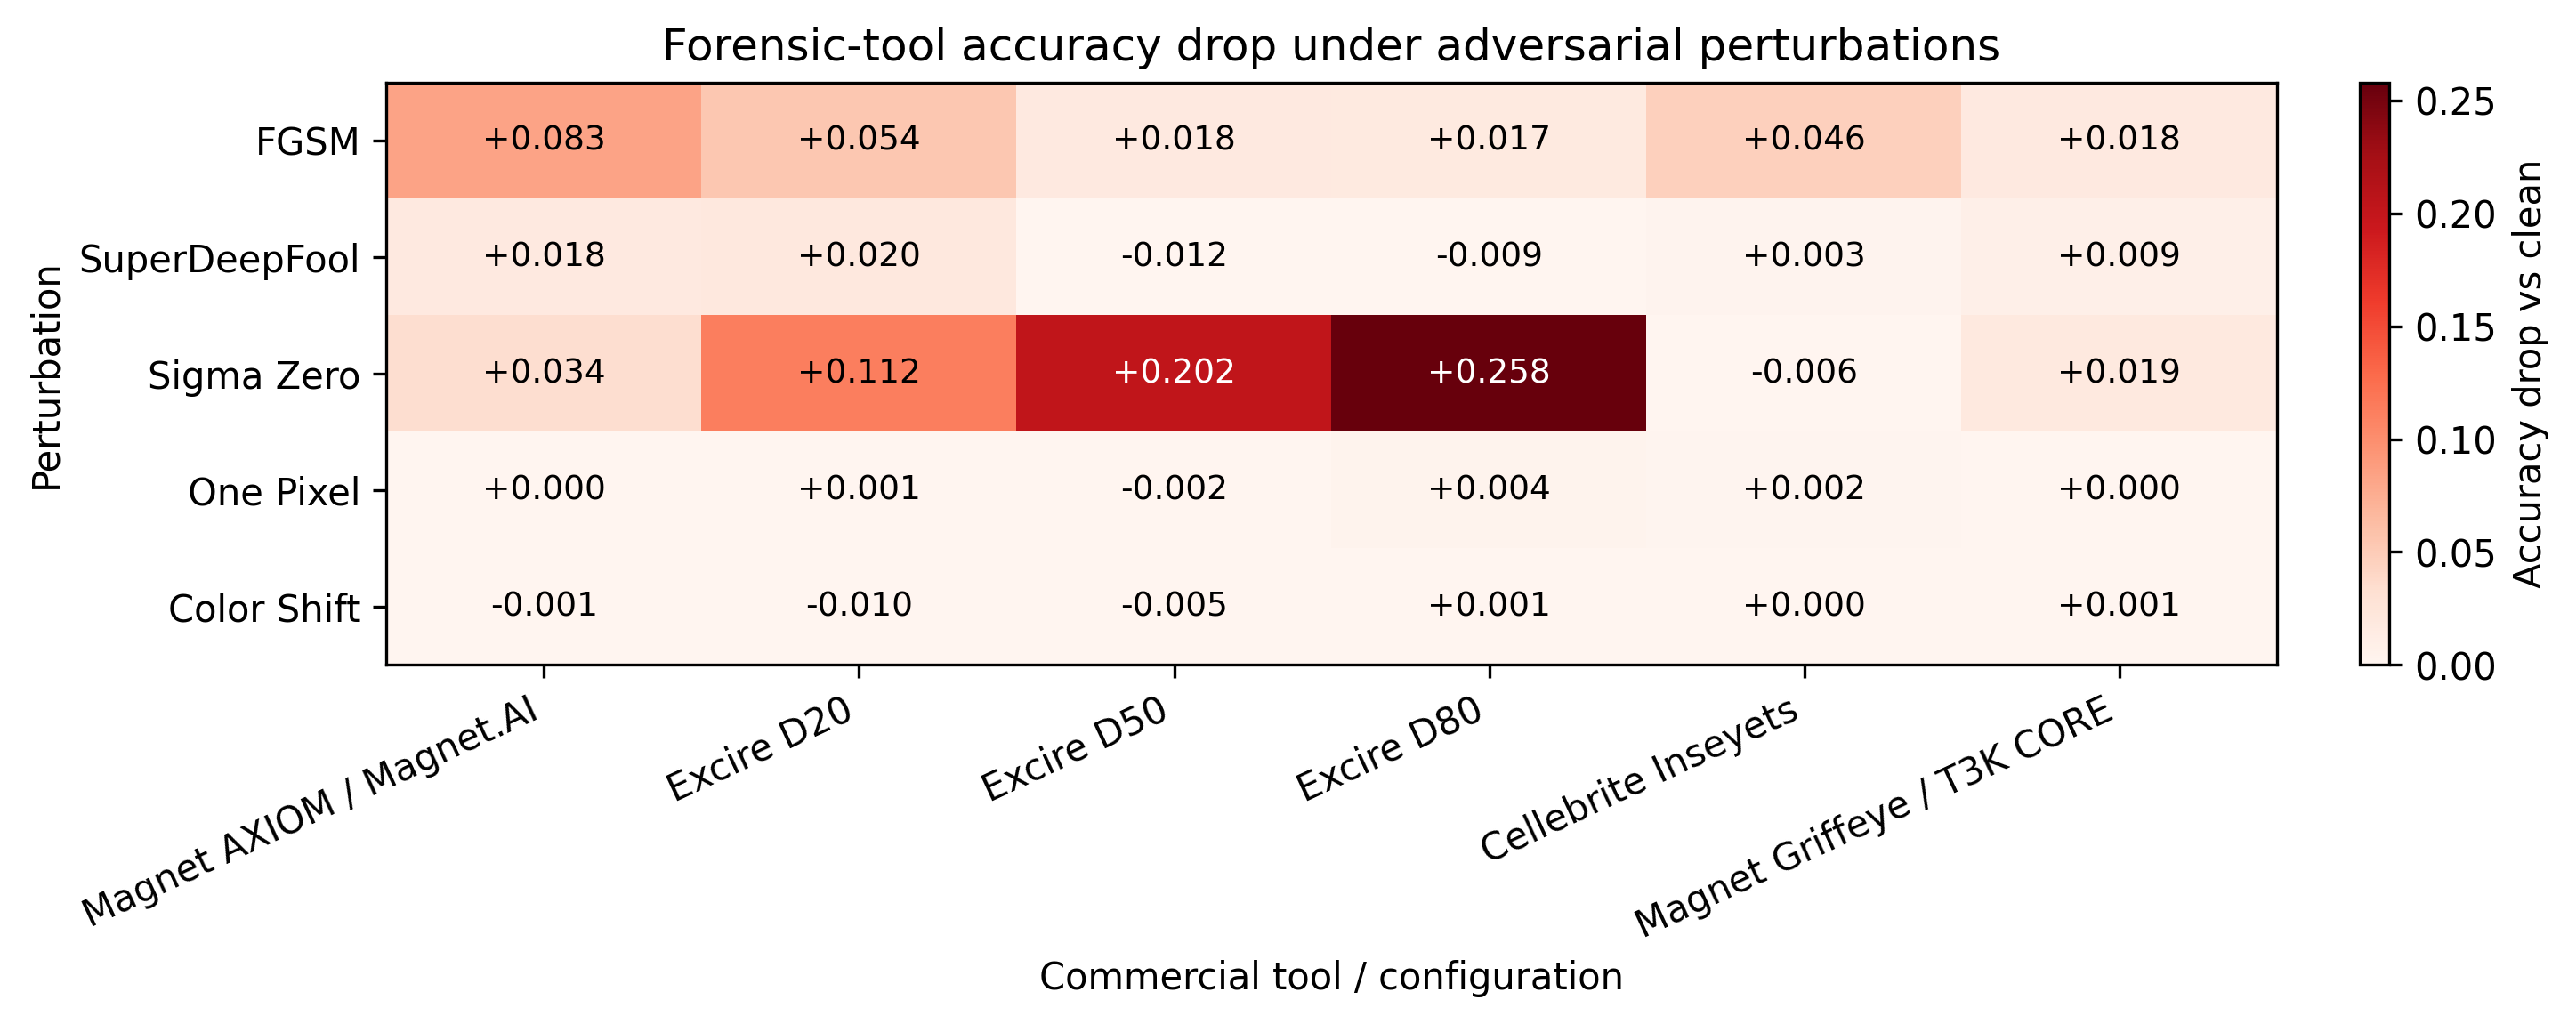
\includegraphics[width=12.60cm,trim=0 0 0 22,clip]{../../results/figures/chapter_5/fig_forensic_tools_adversarial_accuracy_drop_heatmap.png}

\vspace{-0.20cm}
\begin{colorblock}[black]{sintefred!10}{Largest observed accuracy drops}
  \centering\normalsize\bfseries
  Sigma Zero transfer: Excire D50 $20.2$ pp \enspace·\enspace D80 $25.8$ pp
\end{colorblock}
\vspace{-0.12cm}
\centering{\scriptsize\bfseries\color{maincolor}
Empirical transfer from EfficientNet-B0 artifacts---not direct attacks on proprietary models.}
\slideNote
  {Use the publication heatmap to show heterogeneous transfer: the same generated artifact family can affect tools and configurations very differently.}
  {\url{../../results/figures/chapter_5/fig_forensic_tools_adversarial_accuracy_drop_heatmap.png}\par
   \url{../../results/figures/chapter_5/tab_forensic_tools_worst_cases.csv}\par
   Publication package: \texttt{DFRWS\_27/sections/images/heatmap\_blackbox.png}}
\end{frame}

% 09 — Black-box profiles
\begin{frame}{A lower miss rate can create a larger review burden}
\centering
\begin{tikzpicture}[x=1cm,y=1cm]
  \node[font=\scriptsize,text=black!60] at (-1.90,2.63)
    {Clean-condition directional error rates};

  \foreach \p in {0,5,10,15} {
    \pgfmathsetmacro{\xx}{-4.55+\p*0.38}
    \draw[black!12] (\xx,-2.02) -- (\xx,2.35);
    \node[font=\tiny,text=black!55] at (\xx,-2.24) {\p\%};
  }

  \foreach \label/\y/\fnr/\fpr in {
    Magnet.AI/2.05/7.0/3.0,
    Excire D20/1.35/12.0/2.6,
    Excire D50/0.65/4.2/7.0,
    Excire D80/-0.05/1.4/15.6,
    Cellebrite/-0.75/3.2/4.0,
    Griffeye--T3K/-1.45/3.6/0.8} {
      \pgfmathsetmacro{\fnrw}{\fnr*0.38}
      \pgfmathsetmacro{\fprw}{\fpr*0.38}
      \node[font=\tiny,anchor=east,text=black!65] at (-4.75,\y) {\label};
      \fill[sintefred!88] (-4.55,\y+0.06) rectangle (-4.55+\fnrw,\y+0.27);
      \fill[sintefyellow!88!black] (-4.55,\y-0.25) rectangle (-4.55+\fprw,\y-0.04);
      \node[font=\tiny\bfseries,anchor=west] at (-4.45+\fnrw,\y+0.17) {\fnr\%};
      \node[font=\tiny\bfseries,anchor=west] at (-4.45+\fprw,\y-0.15) {\fpr\%};
  }

  \fill[sintefred!88] (-3.30,-2.62) rectangle (-3.05,-2.41);
  \node[font=\tiny,anchor=west] at (-2.95,-2.51) {FNR · missed-target risk};
  \fill[sintefyellow!88!black] (-0.45,-2.62) rectangle (-0.20,-2.41);
  \node[font=\tiny,anchor=west] at (-0.10,-2.51) {FPR · review workload};

  \node[darkpanel,minimum width=4.05cm,minimum height=4.45cm] at (4.18,0.15) {};
  \node[font=\small\bfseries,text=sintefgreen] at (4.18,1.88) {EXCIRE D20 $\rightarrow$ D80};
  \node[font=\Large\bfseries,text=white] at (4.18,1.18) {12.0\% $\rightarrow$ 1.4\%};
  \node[font=\scriptsize,text=white!78] at (4.18,0.80) {missed-target rate};
  \draw[white!30] (2.72,0.32) -- (5.64,0.32);
  \node[font=\Large\bfseries,text=white] at (4.18,-0.20) {2.6\% $\rightarrow$ 15.6\%};
  \node[font=\scriptsize,text=white!78] at (4.18,-0.58) {false-positive rate};
  \draw[white!30] (2.72,-1.06) -- (5.64,-1.06);
  \node[font=\Large\bfseries,text=white] at (4.18,-1.52) {23.8\% $\rightarrow$ 52.2\%};
  \node[font=\scriptsize,text=white!78] at (4.18,-1.90) {OOD weapon assignment};
\end{tikzpicture}
\slideNote
  {Use Excire D20 and D80 to explain that lowering missed targets can sharply increase review workload and OOD routing.}
  {\url{../../results/figures/chapter_5/tab_forensic_tools_clean_metrics.csv}\par
   \url{../../results/figures/chapter_5/tab_forensic_tools_ood_metrics.csv}}
\end{frame}

% 10 — OOD
\begin{frame}{OOD images were still routed to weapon}
\centering
\begin{tikzpicture}[x=1cm,y=1cm]
  \node[font=\scriptsize,text=black!60] at (-1.85,2.70)
    {Weapon-assignment rate on the separate 500-image OOD branch};

  \foreach \p in {0,30,60,90} {
    \pgfmathsetmacro{\xx}{-4.40+\p*0.065}
    \draw[black!12] (\xx,-2.16) -- (\xx,2.42);
    \node[font=\tiny,text=black!55] at (\xx,-2.36) {\p\%};
  }

  \foreach \label/\y/\value/\barcolor in {
    Griffeye--T3K/2.15/26.0/sintefgreen!65!black,
    Cellebrite/1.62/29.2/sintefgreen!65!black,
    Excire D80/1.09/52.2/sintefyellow!88!black,
    Excire D50/0.56/34.0/sintefgreen!65!black,
    Excire D20/0.03/23.8/sintefgreen!65!black,
    Magnet.AI/-0.50/36.0/sintefgreen!65!black,
    CLIP proxy/-1.03/83.6/sintefred!88,
    ResNet18/-1.56/43.8/maincolor,
    EfficientNet-B0/-2.09/37.0/maincolor} {
      \pgfmathsetmacro{\barw}{\value*0.065}
      \node[font=\tiny,anchor=east,text=black!65] at (-4.60,\y) {\label};
      \fill[\barcolor] (-4.40,\y-0.16) rectangle (-4.40+\barw,\y+0.16);
      \node[font=\tiny\bfseries,anchor=west] at (-4.30+\barw,\y) {\value\%};
  }

  \node[redpanel,minimum width=3.50cm,minimum height=1.42cm] at (4.25,1.30) {
    {\fontsize{28}{30}\selectfont\bfseries\color{sintefred!90!black}83.6\%}\\[0.05cm]
    {\small\bfseries CLIP proxy}
  };
  \node[amberpanel,minimum width=3.50cm,minimum height=1.42cm] at (4.25,-0.34) {
    {\Large\bfseries\color{sintefyellow!70!black}23.8--52.2\%}\\[0.05cm]
    {\small\bfseries black-box range}
  };
  \node[font=\scriptsize\bfseries,text=maincolor,align=center,text width=3.6cm] at (4.25,-1.75) {
    Closed-set operating behavior---not a supervised false-positive rate.
  };
\end{tikzpicture}
\slideNote
  {Stress that OOD assignment is reported separately: these images have no supervised weapon/non-weapon ground-truth role.}
  {\url{../../results/metrics/proxy_model_ood_metrics.csv}\par
   \url{../../results/figures/chapter_5/tab_forensic_tools_ood_metrics.csv}}
\end{frame}

% 11 — XAI
\begin{frame}{A maximally concentrated output can still be wrong}
\centering
\begin{tikzpicture}[x=1cm,y=1cm]
  \node[inner sep=0pt] at (-4.70,0.82)
    {
\includegraphics[width=2.62cm]{../LatexThesis/images/fig_xai_case5_adversarial_high_conf_failure_input.png}};
  \node[inner sep=0pt] at (-1.65,0.82)
    {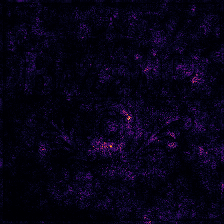
\includegraphics[width=2.62cm]{../LatexThesis/images/fig_xai_case5_adversarial_high_conf_failure_heatmap.png}};
  \node[inner sep=0pt] at (1.40,0.82)
    {
\includegraphics[width=2.62cm]{../LatexThesis/images/fig_xai_case5_adversarial_high_conf_failure_overlay.png}};

  \node[font=\small\bfseries] at (-4.70,-0.84) {Perturbed input};
  \node[font=\scriptsize,text=black!60] at (-4.70,-1.18) {Sigma Zero};
  \node[font=\small\bfseries] at (-1.65,-0.84) {IG magnitude};
  \node[font=\scriptsize,text=black!60] at (-1.65,-1.18) {predicted class};
  \node[font=\small\bfseries] at (1.40,-0.84) {Attribution overlay};
  \node[font=\scriptsize,text=black!60] at (1.40,-1.18) {qualitative only};

  \node[darkpanel,minimum width=3.65cm,minimum height=4.15cm] at (4.75,0.58) {};
  \node[font=\small\bfseries,text=sintefgreen] at (4.75,2.08) {\texttt{xai\_case\_0015}};
  \node[font=\tiny\bfseries,text=white!72] at (4.75,1.47) {REFERENCE};
  \node[font=\small\bfseries,text=white] at (4.75,1.10) {non-weapon};
  \node[font=\tiny\bfseries,text=white!72] at (4.75,0.57) {PREDICTION};
  \node[font=\small\bfseries,text=white] at (4.75,0.20) {weapon};
  \draw[white!30] (3.18,-0.18) -- (6.32,-0.18);
  \node[font=\small\bfseries,text=sintefgreen] at (4.75,-0.55) {MAX-P};
  \node[font=\fontsize{30}{32}\selectfont\bfseries,text=white] at (4.75,-1.08) {1.000};

  \node[greenpanel,minimum width=11.3cm,minimum height=0.88cm,font=\scriptsize\bfseries,text width=10.6cm] at (0,-2.28) {
    Integrated Gradients supports diagnosis of selected proxy outputs. It does not certify correctness, calibrate confidence, or explain proprietary black-box systems.
  };
\end{tikzpicture}
\slideNote
  {Use the case to show that maximum predicted-class probability is not correctness, and that Integrated Gradients remains diagnostic and qualitative.}
  {\url{../LatexThesis/sections/06_results.tex}\par
   \url{../LatexThesis/images/fig_xai_case5_adversarial_high_conf_failure_input.png}\par
   \url{../LatexThesis/images/fig_xai_case5_adversarial_high_conf_failure_heatmap.png}\par
   \url{../LatexThesis/images/fig_xai_case5_adversarial_high_conf_failure_overlay.png}}
\end{frame}

% ---------------------------------------------------------------------
\section{Implications}
% ---------------------------------------------------------------------

% 12 — Workflow
\begin{frame}{AI should prioritize evidence---not exclude it}
\vspace{0.15cm}
\begin{columns}[T,totalwidth=\textwidth]
  \begin{column}{0.235\textwidth}
    \centering{\small\bfseries\color{maincolor}01}\par
    \begin{colorblock}[black]{white}{AI outputs}
      \centering\scriptsize tags · labels\\semantic matches
    \end{colorblock}
  \end{column}
  \begin{column}{0.235\textwidth}
    \centering{\small\bfseries\color{maincolor}02}\par
    \begin{colorblock}[black]{maincolor!7}{Prioritized queue}
      \centering\scriptsize workload reduction\\priority ordering
    \end{colorblock}
  \end{column}
  \begin{column}{0.235\textwidth}
    \centering{\small\bfseries\color{sintefgreen!60!black}03}\par
    \begin{colorblock}[black]{sinteflightgreen}{Human review}
      \centering\scriptsize contextual validation\\expert judgment
    \end{colorblock}
  \end{column}
  \begin{column}{0.235\textwidth}
    \centering{\small\bfseries\color{maincolor}04}\par
    \begin{colorblock}[black]{white}{Documented action}
      \centering\scriptsize defensible forensic\\workflow
    \end{colorblock}
  \end{column}
\end{columns}

\vspace{0.42cm}
\centering{\small\bfseries\color{maincolor}TRACE EVERY DECISION}\par
\vspace{0.20cm}
\begin{columns}[T,totalwidth=0.93\textwidth]
  \begin{column}{0.23\textwidth}\centering\small\bfseries tool version\end{column}
  \begin{column}{0.23\textwidth}\centering\small\bfseries configuration\end{column}
  \begin{column}{0.23\textwidth}\centering\small\bfseries output mapping\end{column}
  \begin{column}{0.23\textwidth}\centering\small\bfseries validation context\end{column}
\end{columns}

\vfill
\begin{colorblock}[white]{maincolor}{}
  \centering\large\bfseries
  Use AI to prioritize evidence review---never to silently exclude it.
\end{colorblock}
\slideNote
  {Translate the findings into a human-in-the-loop rule: prioritization is acceptable; silent exclusion is not.}
  {\url{../LatexThesis/sections/07_conclusions.tex}\par
   \url{../LatexThesis/sections/04_methodology.tex}}
\end{frame}

% 13 — Closing
\begingroup
\setbeamercolor{background canvas}{bg=maincolor}
\setbeamertemplate{headline}{}
\setbeamertemplate{footline}{}
\begin{frame}[plain]
\begin{tikzpicture}[remember picture,overlay]
  \node[anchor=north west,text=white,text width=11.8cm,font=\fontsize{22}{26}\selectfont\bfseries]
    at ([xshift=0.90cm,yshift=-0.72cm]current page.north west)
    {AI can prioritize evidence;\\it must not silently exclude it.};

  \draw[sintefgreen,line width=3pt]
    ([xshift=0.90cm,yshift=-2.40cm]current page.north west) --
    ([xshift=3.55cm,yshift=-2.40cm]current page.north west);

  \node[anchor=north west,text=sintefgreen,font=\Large\bfseries]
    at ([xshift=0.90cm,yshift=-2.82cm]current page.north west) {01};
  \node[anchor=north west,text=white,text width=11.4cm,font=\normalsize\bfseries]
    at ([xshift=1.85cm,yshift=-2.82cm]current page.north west)
    {Clean performance is only a baseline; robustness depends on the condition.};

  \node[anchor=north west,text=sintefgreen,font=\Large\bfseries]
    at ([xshift=0.90cm,yshift=-4.05cm]current page.north west) {02};
  \node[anchor=north west,text=white,text width=11.4cm,font=\normalsize\bfseries]
    at ([xshift=1.85cm,yshift=-4.05cm]current page.north west)
    {Direct attacks, transfer and OOD behavior are distinct from\\configuration trade-offs.};

  \node[anchor=north west,text=sintefgreen,font=\Large\bfseries]
    at ([xshift=0.90cm,yshift=-5.58cm]current page.north west) {03};
  \node[anchor=north west,text=white,text width=11.4cm,font=\normalsize\bfseries]
    at ([xshift=1.85cm,yshift=-5.58cm]current page.north west)
    {FAIRLab makes those dimensions traceable and auditable for a forensic expert.};

  \node[anchor=north west,text=white,font=\Large\bfseries]
    at ([xshift=0.90cm,yshift=-8.02cm]current page.north west) {Questions};
  \node[anchor=north east,text=white!65,font=\scriptsize]
    at ([xshift=-0.90cm,yshift=-8.10cm]current page.north east) {Backup slides follow};

  \node[anchor=north east]
    at ([xshift=-0.95cm,yshift=-0.55cm]current page.north east)
    {
\includegraphics[width=1.55cm]{assets/logo_RGB.png}};
\end{tikzpicture}
\slideNote
  {Close by returning to the operational question. Pause after the final sentence and invite questions.}
  {\url{../LatexThesis/sections/07_conclusions.tex}}
\end{frame}
\endgroup

% ---------------------------------------------------------------------
\appendix
\section{Backup}
% ---------------------------------------------------------------------

% 14 — Backup RQs
\begin{frame}{Research questions and claim scope}
\centering
\begin{tikzpicture}[x=1cm,y=1cm]
  \node[font=\Large\bfseries,text=maincolor,anchor=west] at (-6.10,2.30) {RQ1};
  \node[font=\small,anchor=west,text width=10.7cm] at (-4.55,2.30)
    {To what extent do the proxy models retain clean-baseline performance across separate OOD, adversarial and anti-forensic conditions?};
  \draw[black!12] (-4.55,1.68) -- (6.15,1.68);

  \node[font=\Large\bfseries,text=maincolor,anchor=west] at (-6.10,1.15) {RQ2};
  \node[font=\small,anchor=west,text width=10.7cm] at (-4.55,1.15)
    {How do direct source-model attacks, cross-architecture transfer and model-agnostic Color Shift differ?};
  \draw[black!12] (-4.55,0.55) -- (6.15,0.55);

  \node[font=\Large\bfseries,text=maincolor,anchor=west] at (-6.10,0.02) {RQ3};
  \node[font=\small,anchor=west,text width=10.7cm] at (-4.55,0.02)
    {How do black-box outputs and configuration choices shape the observed operational profiles?};
  \draw[black!12] (-4.55,-0.58) -- (6.15,-0.58);

  \node[font=\Large\bfseries,text=maincolor,anchor=west] at (-6.10,-1.12) {RQ4};
  \node[font=\small,anchor=west,text width=10.7cm] at (-4.55,-1.12)
    {Which directional errors, degradations, OOD assignments and unknown states matter for continued human review?};

  \node[softpanel,minimum width=10.8cm,minimum height=0.68cm,font=\scriptsize\bfseries,text width=10.2cm] at (0,-2.35) {
    Scope: operational robustness under the frozen protocol---not certification, legal admissibility or universal ranking.
  };
\end{tikzpicture}
\slideNote
  {Use this slide if the commission asks for the exact research questions or the formal scope of the claim.}
  {\url{../LatexThesis/sections/01_introduction.tex}\par
   \url{../LatexThesis/sections/07_conclusions.tex}}
\end{frame}

% 15 — Backup perturbations
\begin{frame}{Perturbation suite and evaluation paths}
\vspace{0.12cm}
\begin{columns}[T,totalwidth=0.96\textwidth]
  \begin{column}{0.47\textwidth}
    \begin{colorblock}[black]{sintefred!10}{Adversarial / adversarial-style}
      \small
      \begin{itemize}
        \item FGSM
        \item One Pixel
        \item Sigma Zero
        \item SuperDeepFool
        \item Color Shift
      \end{itemize}
    \end{colorblock}
  \end{column}
  \begin{column}{0.47\textwidth}
    \begin{colorblock}[black]{sinteflightgreen}{Anti-forensic transformations}
      \small
      \begin{itemize}
        \item JPEG recompression
        \item Resample / resize
        \item Gaussian blur
        \item Histogram modification
        \item Contrast stretching
      \end{itemize}
    \end{colorblock}
  \end{column}
\end{columns}

\vspace{0.12cm}
\begin{colorblock}[white]{maincolor}{Evaluation path}
  \centering\scriptsize\bfseries
  Model-dependent attacks: direct on EfficientNet-B0 · empirical transfer elsewhere\\[0.04cm]
  Color Shift and anti-forensic transformations: model-agnostic conditions
\end{colorblock}
\slideNote
  {Use if asked which perturbations were included and which threat-model path applies to each family.}
  {\url{../LatexThesis/sections/04_methodology.tex}\par
   \url{../LatexThesis/sections/05_implementation.tex}}
\end{frame}

% 16 — Backup table
\begin{frame}{Commercial clean metrics and OOD behavior}
\centering
\small
\setlength{\tabcolsep}{5.2pt}
\renewcommand{\arraystretch}{1.28}
\rowcolors{2}{maincolor!6}{white}
\begin{tabular}{>{\bfseries}lccccc}
  \rowcolor{maincolor}
  \color{white}Configuration &
  \color{white}Accuracy &
  \color{white}Recall &
  \color{white}FNR &
  \color{white}FPR &
  \color{white}OOD W-rate \\
  Magnet.AI          & 95.0\% & 93.0\% & 7.0\%  & 3.0\%  & 36.0\% \\
  Excire D20         & 92.7\% & 88.0\% & 12.0\% & 2.6\%  & 23.8\% \\
  Excire D50         & 94.4\% & 95.8\% & 4.2\%  & 7.0\%  & 34.0\% \\
  Excire D80         & 91.5\% & 98.6\% & 1.4\%  & 15.6\% & 52.2\% \\
  Cellebrite Inseyets& 96.4\% & 96.8\% & 3.2\%  & 4.0\%  & 29.2\% \\
  Griffeye / T3K     & 97.8\% & 96.4\% & 3.6\%  & 0.8\%  & 26.0\%
\end{tabular}

\vspace{0.35cm}
\begin{colorblock}[black]{sintefyellow!22}{Interpretation boundary}
\centering\small
Interpret the rows as frozen operating profiles; the metrics do not establish a universal product ranking.
\end{colorblock}
\slideNote
  {Use for exact clean and OOD figures. Remind the commission that versions, configurations and mappings are frozen protocol conditions.}
  {\url{../../results/figures/chapter_5/tab_forensic_tools_clean_metrics.csv}\par
   \url{../../results/figures/chapter_5/tab_forensic_tools_ood_metrics.csv}}
\end{frame}

% 17 — Backup traceability
\begin{frame}{Traceability links sources to reported figures}
\vspace{0.25cm}
\begin{columns}[T,totalwidth=\textwidth]
  \begin{column}{0.19\textwidth}
    \begin{colorblock}[black]{white}{Source}
      \centering\scriptsize manifests\\manual review
    \end{colorblock}
  \end{column}
  \begin{column}{0.19\textwidth}
    \begin{colorblock}[black]{maincolor!7}{Derivation}
      \centering\scriptsize splits · attacks\\source IDs
    \end{colorblock}
  \end{column}
  \begin{column}{0.19\textwidth}
    \begin{colorblock}[black]{sinteflightgreen}{Decision}
      \centering\scriptsize predictions\\normalized outputs
    \end{colorblock}
  \end{column}
  \begin{column}{0.19\textwidth}
    \begin{colorblock}[black]{maincolor!7}{Metric}
      \centering\scriptsize condition tables\\directional errors
    \end{colorblock}
  \end{column}
  \begin{column}{0.19\textwidth}
    \begin{colorblock}[black]{white}{Report}
      \centering\scriptsize thesis figures\\conclusion tables
    \end{colorblock}
  \end{column}
\end{columns}

\vspace{0.45cm}
\centering{\large\bfseries\color{maincolor}Integrity and audit controls}\par
\vspace{0.15cm}
\begin{minipage}{0.86\textwidth}
\small
\begin{itemize}
  \item SHA-256 digests for datasets, bundles, checkpoints and controlled artifacts
  \item Frozen model, tool-version and configuration registries
  \item Explicit output-normalization rules and unmatched/unknown handling
  \item Repository scripts regenerate metrics and thesis-ready reporting assets
\end{itemize}
\end{minipage}
\slideNote
  {Use if asked how a reported figure can be traced back to its source item and tool output.}
  {\url{../artifact/THESIS_ARTIFACT.md}\par
   \url{../artifact/REPRODUCIBILITY.md}\par
   \url{../artifact/CONTROLLED_ARTIFACT_CHECKSUMS.sha256}}
\end{frame}

% 18 — Backup claim boundaries
\begin{frame}{Claim boundaries keep the result defensible}
\centering
\begin{tikzpicture}[x=1cm,y=1cm]
  \node[darkpanel,minimum width=4.50cm,minimum height=4.55cm] at (-4.38,0.20) {};
  \node[font=\scriptsize\bfseries,text=sintefgreen] at (-4.38,1.98) {METADATA SENSITIVITY};
  \node[font=\fontsize{30}{32}\selectfont\bfseries,text=white] at (-4.38,1.27) {15};
  \node[font=\scriptsize\bfseries,text=white] at (-4.38,0.72) {of 11,500 files};
  \node[font=\scriptsize,text=white!80,align=center,text width=3.75cm] at (-4.38,0.20) {
    matched a predefined\\sensitive metadata term
  };
  \draw[white!30] (-5.80,-0.28) -- (-2.96,-0.28);
  \node[font=\scriptsize\bfseries,text=white,align=center,text width=3.80cm] at (-4.38,-0.78) {
    Leave-out differences\\were small
  };
  \node[font=\scriptsize,text=sintefyellow!58,align=center,text width=3.80cm] at (-4.38,-1.60) {
    This does not prove causal\\irrelevance for every decision.
  };

  \node[font=\small\bfseries,text=maincolor,anchor=west] at (-1.45,2.45) {CLAIM BOUNDARIES};

  \node[font=\scriptsize\bfseries,text=maincolor,anchor=west] at (-1.45,1.72) {Corpus};
  \node[font=\scriptsize,anchor=west,text width=5.15cm] at (0.55,1.72)
    {1,500 images; one reviewer};
  \draw[black!12] (-1.45,1.30) -- (6.25,1.30);

  \node[font=\scriptsize\bfseries,text=maincolor,anchor=west] at (-1.45,0.92) {Perturbations};
  \node[font=\scriptsize,anchor=west,text width=5.15cm] at (0.55,0.92)
    {one frozen setting per condition};
  \draw[black!12] (-1.45,0.50) -- (6.25,0.50);

  \node[font=\scriptsize\bfseries,text=maincolor,anchor=west] at (-1.45,0.12) {Attack target};
  \node[font=\scriptsize,anchor=west,text width=5.15cm] at (0.55,0.12)
    {direct attacks only on \mbox{EfficientNet-B0}};
  \draw[black!12] (-1.45,-0.30) -- (6.25,-0.30);

  \node[font=\scriptsize\bfseries,text=maincolor,anchor=west] at (-1.45,-0.68) {Black-box};
  \node[font=\scriptsize,anchor=west,text width=5.15cm] at (0.55,-0.68)
    {tool version + settings + mapping};
  \draw[black!12] (-1.45,-1.10) -- (6.25,-1.10);

  \node[font=\scriptsize\bfseries,text=sintefred!90!black,anchor=west] at (-1.45,-1.48) {Legal scope};
  \node[font=\scriptsize,anchor=west,text width=5.15cm] at (0.55,-1.48)
    {operational triage only; no legal claim};

  \node[softpanel,minimum width=7.55cm,minimum height=0.65cm,
        font=\scriptsize\bfseries,text width=6.90cm] at (2.38,-2.34) {
    Protocol-specific assessment---not certification or universal ranking.
  };
\end{tikzpicture}
\slideNote
  {Use if asked about metadata leakage, external validity or the strongest limitation of the protocol.}
  {\url{../../results/figures/chapter_5/embedded_metadata_sensitivity_summary.json}\par
   \url{../LatexThesis/sections/06_results.tex}\par
   \url{../LatexThesis/sections/07_conclusions.tex}}
\end{frame}

\end{document}
